\documentclass[conference,compsoc]{IEEEtran}
\newcommand\tab[1][0.75cm]{\hspace*{#1}}
\usepackage[utf8]{inputenc}

%\ifCLASSOPTIONcompsoc
   \usepackage[nocompress]{cite}
%\else
 
\usepackage{cite}
\usepackage{url}
%\fi


\usepackage[pdftex]{hyperref}


% *** GRAPHICS RELATED PACKAGES ***

\ifCLASSINFOpdf
   \usepackage{graphicx}
   \graphicspath{{files/}}
  
\else
 
\fi
% correct bad hyphenation here
\hyphenation{op-tical net-works semi-conduc-tor}

%********** Começo do documento ************88

\begin{document}



\title{\resizebox{!}{0.75cm}{Ponto de controle 1}\\Monitoramento facial em tempo real aplicado no Restaurante Universitário da Faculdade Gama.}



\author{
\IEEEauthorblockN{João Vitor Rodrigues Baptista}
\IEEEauthorblockA{15/0013329\\UnB - FGA \\
Brasília, Brasil \\
Email: jvrbaptista@live.com }
\and
\IEEEauthorblockN{Igor Sousa Nunes de Oliveira}
\IEEEauthorblockA{15/0011971\\
UnB - FGA \\
Brasília, Brasil\\
Email: igorsno97@gmail.com }}
\maketitle

% As a general rule, do not put math, special symbols or citations
% in the abstract

\begin{abstract}
Aplicação de monitoramento facial em tempo real no Restaurante Universitário da Faculdade Gama utilizando Raspberry pi para melhorar a eficiência do sistema e evitando problemas no acesso de usuários. \cite{referencia:3} 
\end{abstract}
\IEEEpeerreviewmaketitle
\section{Introdução}
Sistemas de controles de acesso são uma ferramenta muito importante na contemporaneidade para a segurança de ambientes controlados, produtos, pessoas ou para de maneira simples um controle de tempo dos usuários do sistema. \cite{referencia:7}

A partir disso foi observado uma grande ineficiência no sistema de controle do Restaurante Universitário da Faculdade Gama. Com constantes falhas no sistema que gera filas gigantescas como: sistema fora do ar - onde todo o controle passa a ser feito manualmente -, lentidão no acesso e a necessidade de um funcionário para verificar as a identidade dos alunos manualmente. 

%Muitos sistemas de identificação e controle de ambientes se tornaram de uso comum e amplo em diversas áreas, desde passes de ônibus ou mesmo pontos eletrônicos para registro de horas trabalhadas, esse tipo de ferramenta  de controle de acesso pode ser de maneira simples dividida em duas etapas, sendo a primeira uma etapa de verificação ou identificação, que pode ser feita através de cartões, senhas digitadas pelo usuário, códigos de barra ou mesmo códigos do tipo "QR".

%Com o passar do tempo notou-se que uma boa forma de identificação seria através de padrões do ser humano de maneira que a chave de acesso sempre estaria com usuário. Um dos padrões bastante associados com a identificação foi a digital, e desde cedo estudada para se entender padrões já que a  mesma é diferente para cada pessoa, sensores biométricos se tornaram bastante utilizados desde celulares até mesmo cofres. Um padrão que está sobre um grande estudo na contemporaneidade são padrões reconhecidos por imagem como a face e em certas aplicações até mesmo a leitura de padrões na iris do usuários.\cite{referencia:7}

A tecnologia entrou em um padrão de evolução buscando maior conforto, acessibilidade, velocidade e segurança
para seus usuários, o reconhecimento facial se tornou uma poderosa ferramenta na aquisição de dados por 
não precisar de módulos sensores de uso específicos como o leitor biométrico. 

Em países como a China onde o investimento na área de segurança e processamento digital de imagens conseguiram criar uma rede de câmeras que identificam pessoas a distancia, então o processo de transformar o usuário na própria chave do sistema
foi a melhor saída para uma maior segurança do sistema, praticidade e até mesmo melhoras no fluxo de filas em 
ambientes controlados entre outros.\cite{referencia:4} \cite{referencia:5} 
\section{Justificativa}
É de notável visibilidade que filas tendem a obstruir o fluxo de pessoas que tem a intenção de passar entre passagens principalmente em áreas ou ambientes que possuem controle de entrada ou alguma possível restrição de acesso, o fluxo de pessoas consegue se tornar maior e mais problemático
principalmente nos lugares que possuem catracas físicas que por meio do bloqueio de fluxo controlem o acesso de pessoas por meio de passes entre outros. Com isso foi verificado que
os meios de identificação podem ser ineficientes quanto a fluidez das
pessoas que transitam esses meios.

Motivado pela lentidão provocada por meios de identificação lentos comumente usadas fez-se necessária uma alternativa de mecanismo que torne essa passagem mais eficiente e fluida para as pessoas, contudo tal alternativa deve ao mesmo tempo atender as necessidades de segurança e controle do ambiente. A segurança é fundamental para verificar as pessoas que adentram um ambiente restrito e possam reconhecer pessoas desconhecidas que possam tentar entrar no lugar, por isso deve ser feito o monitoramento de horários de quem entra e sai do local e deve-se sempre ficar atento a pessoas que possivelmente tentariam entrar no ambiente sem ter autorização.

Com isso,a partir da utilização de reconhecimento facial ficará mais
 cômodo para as pessoas, já que o sistema será mais eficiente e automatizado. Evitando-se assim diversos problemas da utilização de outros meios de identificação  como
cartões(RFIDS, magnéticos  e codigo de barras), senhas digitadas manualmente, 
 
 \section{Objetivos}
Tornar o controle de acesso ao Restaurante Universitário da Faculdade Gama eficientes tornando o fluxo de pessoas que entram mais rápido e automatizando o controle de usuários.
Identificar as pessoas que entram e saem além de poder ter
controle dos tempos de acessos de cada pessoa individualmente e armazenar em um banco de dados.
Monitorar pessoas que tentem entrar no ambiente de forma
indevida e impedir a entrada de usuários quem não tenham a
devida autorização.

 \begin{figure}[!ht]
		\centering
		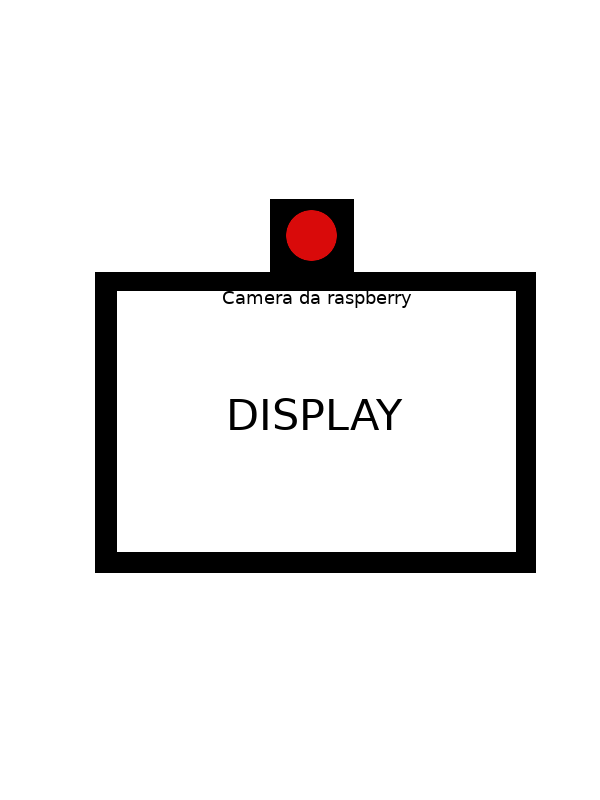
\includegraphics[scale=0.25]{Prototipo.png}
		\caption{Primeira concepção do protótipo.}
		%\label{Rotulo}
\end{figure}
 
\section{Requisitos}
\begin{itemize}
   \item Um microcontrolador no qual a escolha de projeto é o Raspberry pi 3 B. 
   \item Um módulo de câmera para a Raspberry.
   \item Um display para se mostrar as informações necessárias.
   \item Uma estrutura para proteger o sistema(case).
   \item Cabo HDMI.
   \item Modulo rele 12V.
   \item Fonte de tensão.
   \item Conexão com a internet.
   \item Um ambiente onde se possa manter registro de pessoas e de
horários de entrada e saída da mesma para monitoração.(servidor).
 \end{itemize}
 
\section{Benefícios}
Processo com maior segurança para os usuários, onde não é necessário  memorizar senhas ou carregar algum tipo de chave, o traço pessoal é mais dificil de ser clonado ou copiado o que trás maior segurança para todos os usuários do sistema.

O fluxo de pessoas se torna maior e mais eficiente com um método de identificação mais rápido e que não necessita de algum acessório adicional para o funcionamento. Praticidade para o controlador do sistema que tem registro com hora e fotos, e pelo lado das pessoas que convivem com o sistema precisam de pouco tempo para se acostumar com o sistema e além disso trás um maior conforto para as mesmas.
%---------------------  ----------------------

%\section{Materiais Utilizados}
%TABELAS AQUI

%\begin{table}[tbp]
%\caption{Tabela 1 - Exemplo}
%\label{my-label}
%\begin{tabular}{ccccc}
%\textbf{Nome}   & \textbf{Nome1} & \textbf{Nome2} & \textbf{Nome3} & \textbf{Nome4} \\
%\textbf{Nome11} & 1              & 2              & 3              & 4              \\
%\textbf{Nome21} & 5              & 6              & 7              & 8              \\
%\textbf{Nome31} & 9              & 10             & 11             & 12            
%\end{tabular}
%\end{table}
%---------------------  ----------------------

%\section{Hardware e Software}

%---------------------  ----------------------
%\subsection{Descrição do Hardware}

%Como é observado no diagrama de blocos, é necessária uma fonte externa para acionar a trava solenoide, pois os 3 volts fornecidos pela placa não é suficiente para fazer o acionamento da trava.

%\begin{figure}[!ht]
%		\centering
%		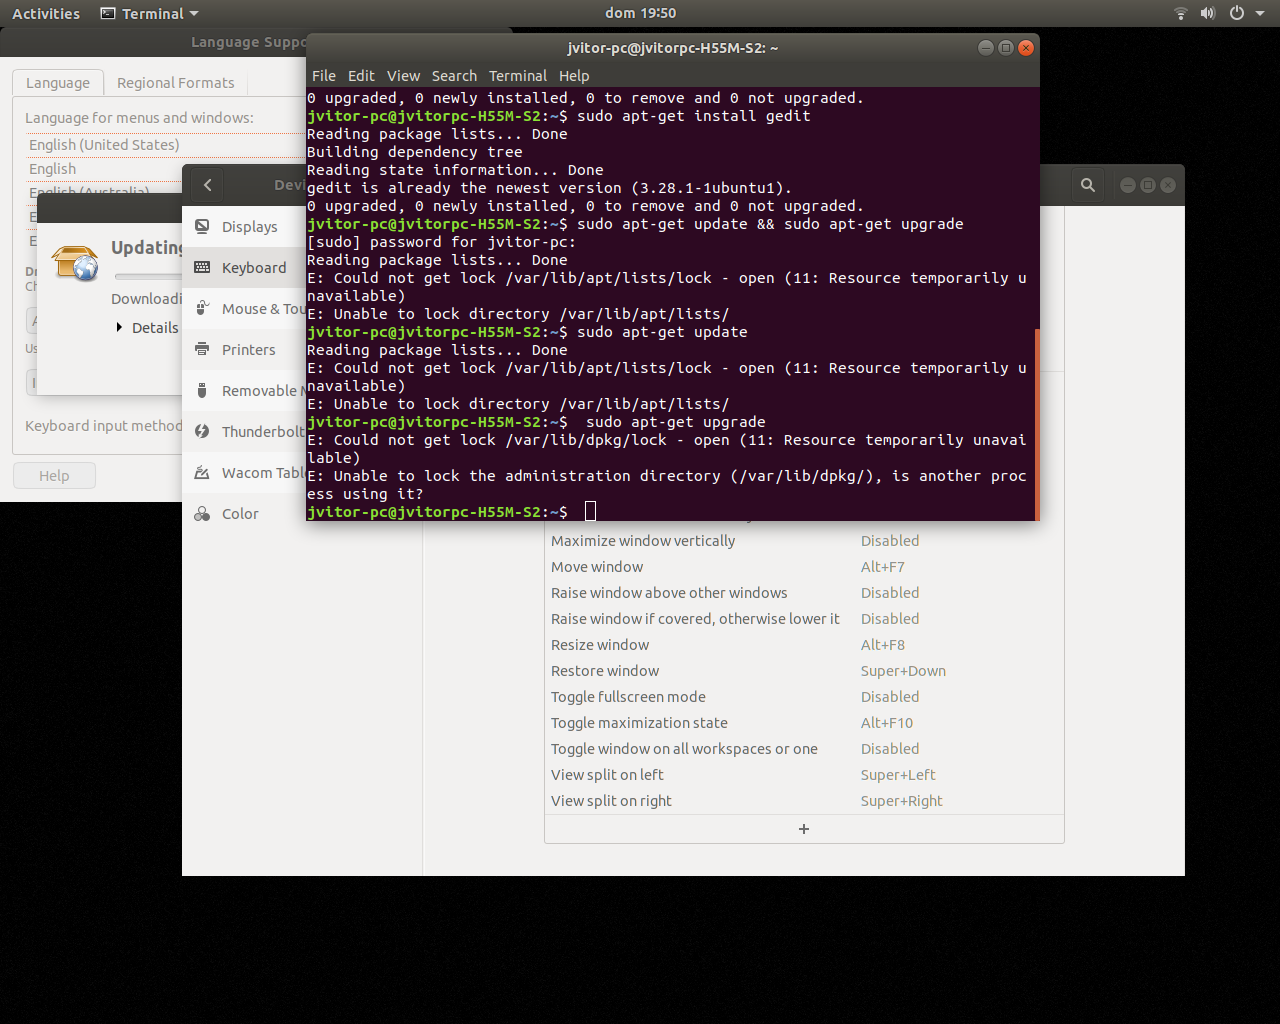
\includegraphics[scale=0.15]{nome_da_figura.png}
%		\caption{Figura 1.}
		%\label{Rotulo}
%\end{figure}

%O resultado foi o esperado, ao passar o tag no leitor RFID, gerou-se um sinal para o relê abrir a tranca eletrônica, através da alimentação de uma bateria de 9 – 12V. 
%Display de Cristal Liquido: Pode ser facilmente implementado no MSP430 utilizando a biblioteca "LiquidCrystal.h". O display será utilizado para exibir as mensagens:

%---------------------  ----------------------


%\subsection{Descrição do Software}
%Para melhor ilustrar o caminho logico deste sistema, foi construído um Diagrama Logico na imagem 5. Para mostrar de maneiras simples a ideia lógica do sistema proposto.
% \begin{figure}[!ht]
%		\centering
%		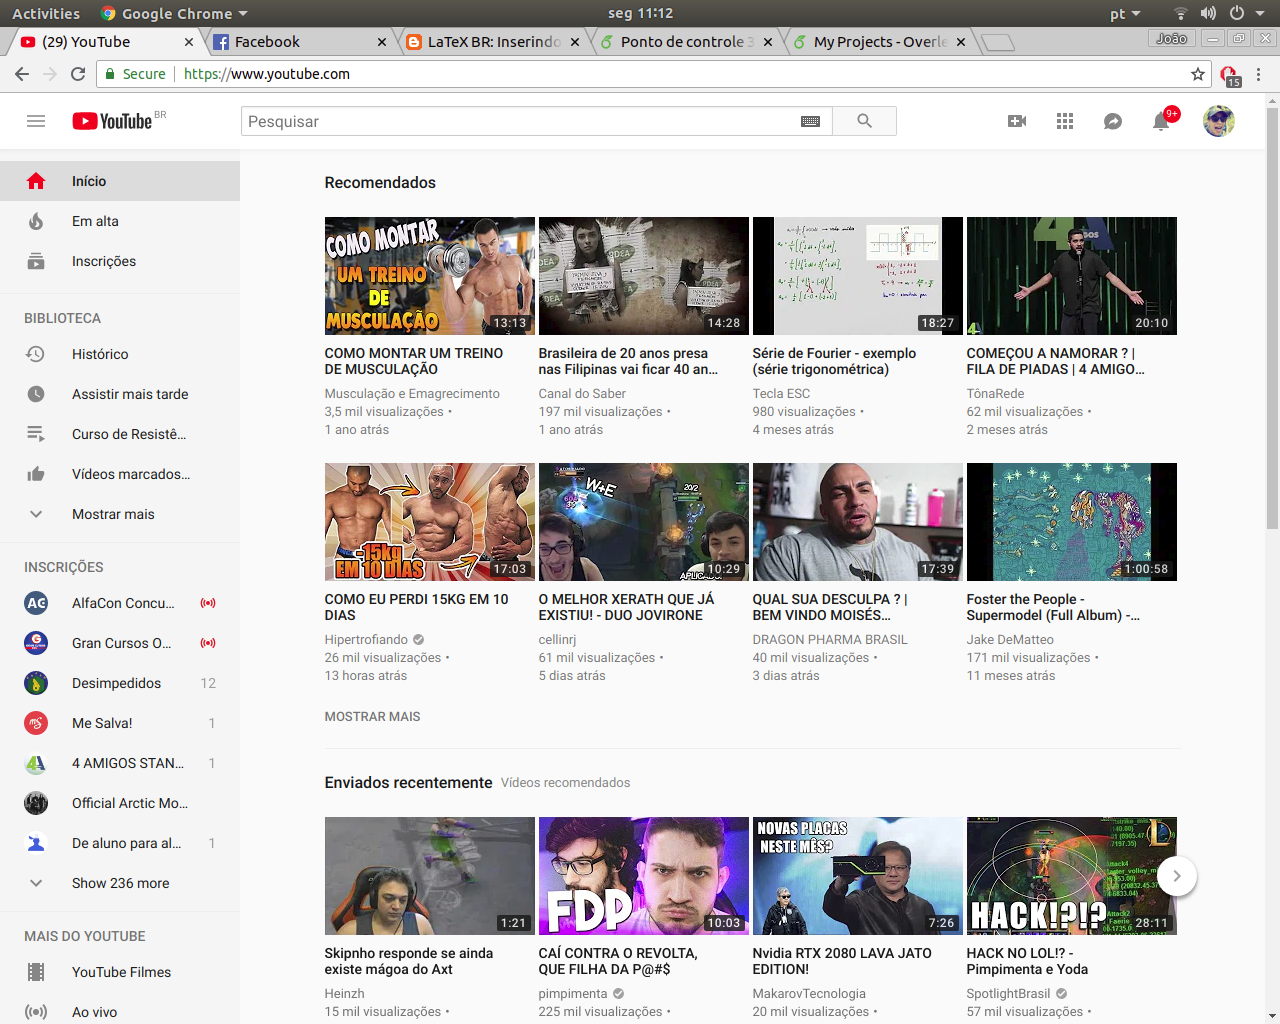
\includegraphics[scale=0.15]{nome_da_figura1.png}
%		\caption{Figura 1}
		%\label{Rotulo}
%\end{figure}

%O Sistema consiste nos seguintes passos:

%\tab 1. Iniciar a comunicação UART com o RC522. Exibindo “RFID LOADING...” ao iniciar.

%\tab 2. Quando o sistema estiver pronto e iniciado exibir “PASSE O CARTÃO”.

%\tab 3. Ler o conteúdo do cartão ou tag.

%\tab 4. Julgar se o cartão ou tag, pode ou não destravar o sistema.

%\tab 5. Destrava o sistema e envia um sinal para o rele, exibe  “BEM VINDO USUARIO”, espera 7 segundos e vai para o loop de leitura.

%\tab 6. Trava o sistema quando o cartão não tem acesso, exibe “ACESSO NEGADO”, volta para o loop de leitura. 



%\begin{figure}[!ht]
%		\centering
%		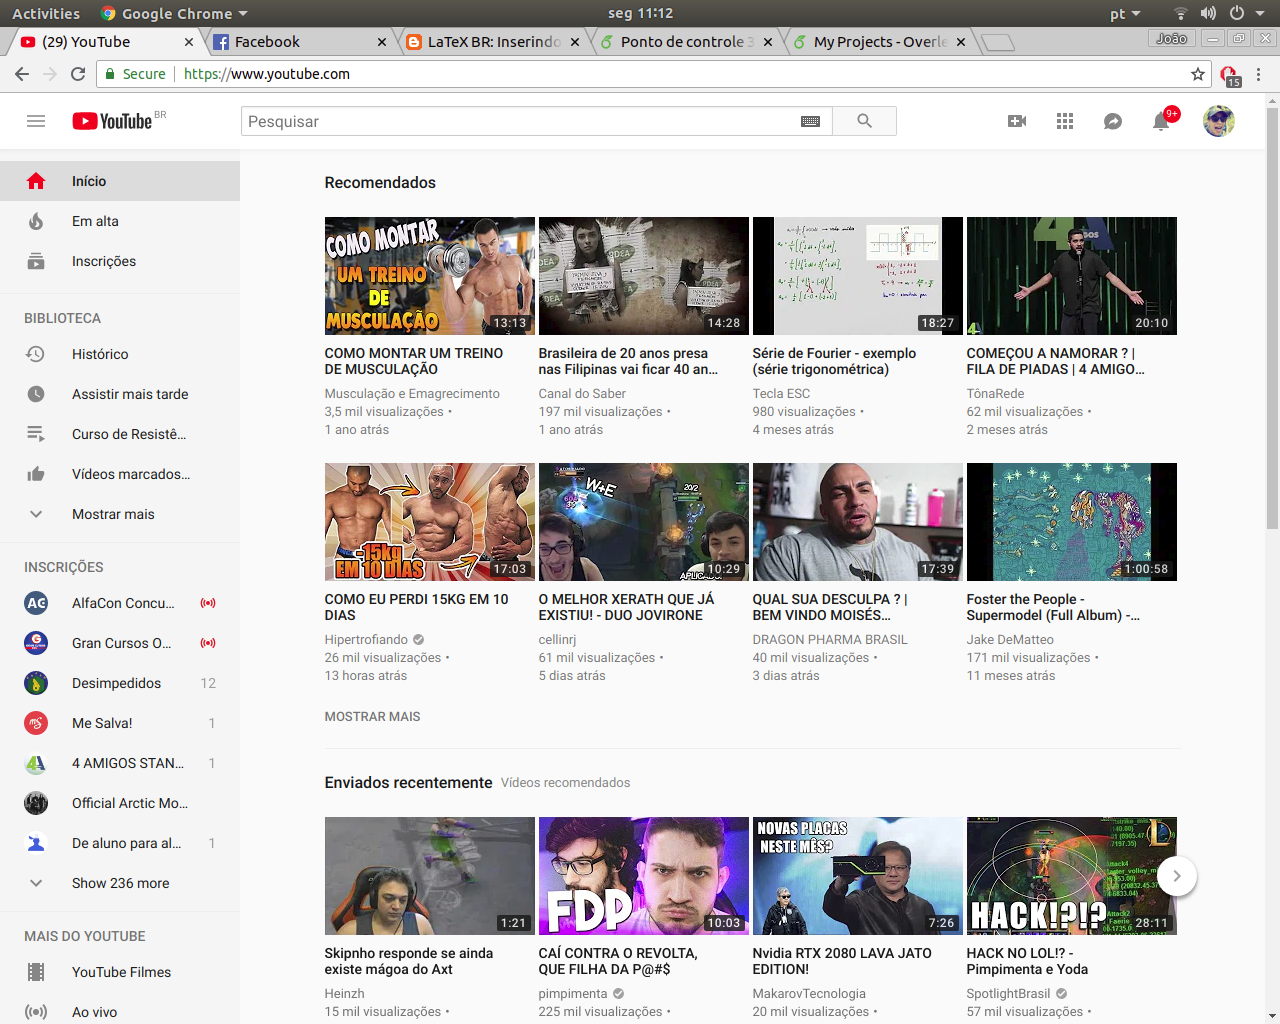
\includegraphics[scale=0.15]{nome_da_figura1.png}
%		\caption{Figura 1}
		%\label{Rotulo}
%\end{figure}

%Os códigos e as figuras estão no GitHub, através do link:\href{https://github.com/helpthx}{https://github.com/helpthx}

%---------------------  ----------------------

%\section{Resultado}
%Os resultados foram conforme o esperado ao se juntar todos os componentes, entretanto houve algum problema na comunicação com o display 16x2, o qual não exibe as mensagens de trava e destrava do sistema de maneira correta, ou seja, em certos momentos caracteres estranhos são mostrados no display. Porem a comunicação entre o RC522, MSP430 e o rele esta totalmente funcional e a trava esta se comportando como deveria. Para os próximos passos será corrigido o problema do display e possivelmente adicionado mais funções ao sistema.

%\begin{figure}[!ht]
%		\centering
%		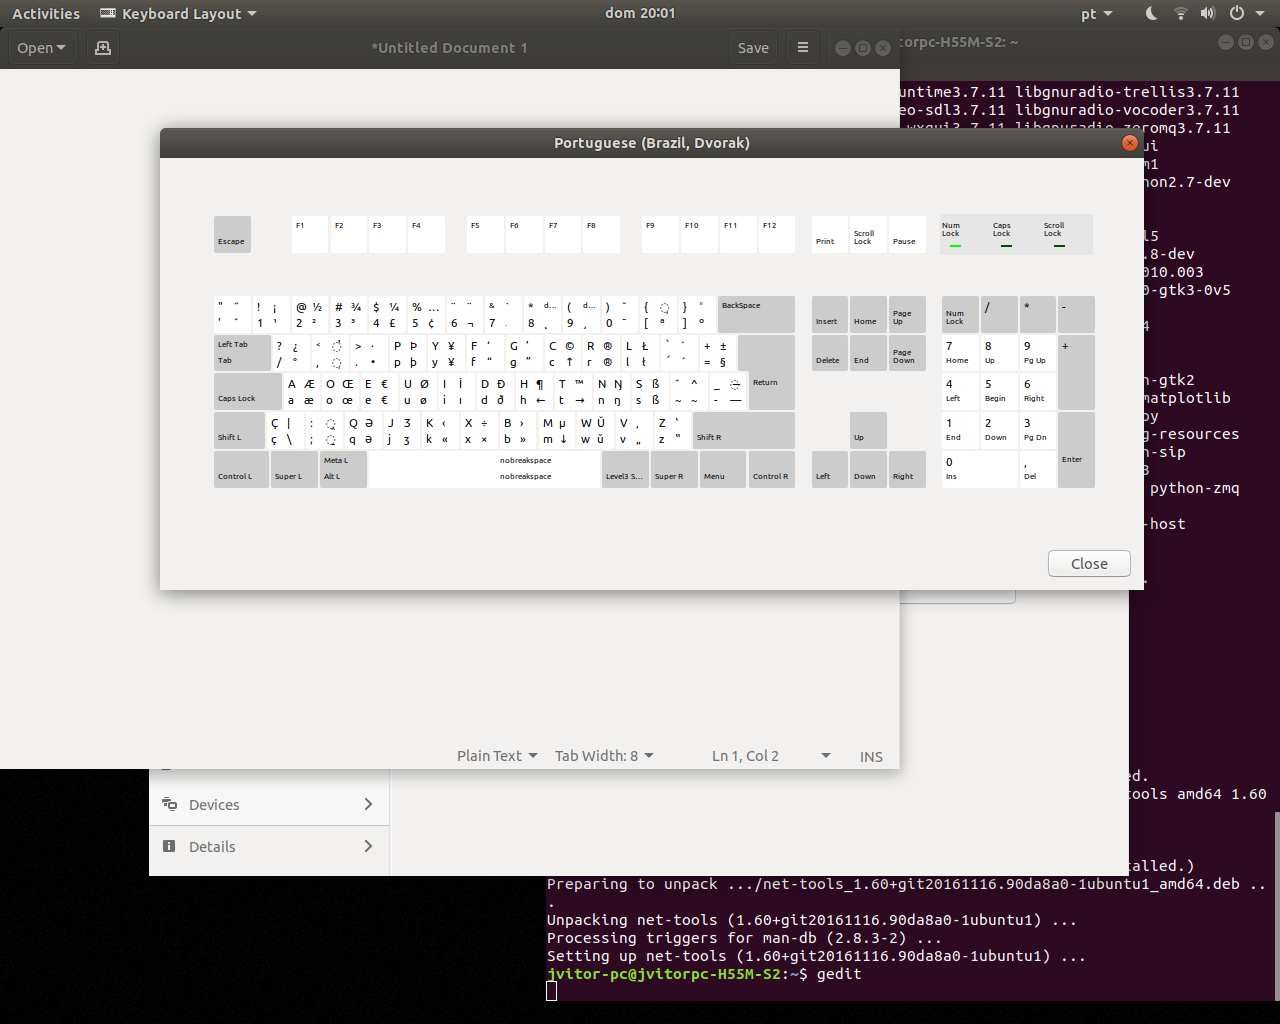
\includegraphics[scale=0.15]{nome_da_figura3.png}
%		\caption{Figura 3}
		%\label{Rotulo}
%\end{figure}

%---------------------  ----------------------

%\section{Relação de Custo}
%Até o presente momento se foi gasto em torno de R\$214,10 para o projeto, o que pode ser extremamente reduzido se as peças fossem compradas com certa antecipação, o MSP comprado direto pelo fornecedor a Texas, dessa maneira fazer com que o preço do projeto reduzido em mais de 50\% do valor atual, os outros componentes se comprando em grandes quantidades consegue-se uma grande redução de preços, o que viabilizaria a construção em maior escala do projeto com um menor preço e com certas melhorias uma possível entrada na concorrência de vendas de produtos pensados para segurança e controle de ambientes, como sendo uma alternativa de baixo custo que poderia ser modificada com necessidades do próprio cliente. \cite{referencia:1}



%-------------------- REFERÊNCIA -----------------

\begin{thebibliography}{1}


%\bibitem{IEEEhowto:kopka}
%H.~Kopka and P.~W. Daly, \emph{A Guide to \LaTeX}, 3rd~ed.\hskip 1em plus
 % 0.5em minus 0.4em\relax Harlow, England: Addison-
%FALTA ARRUMAR AS REFERÊNCIAS


\bibitem{referencia:2}
{TIWARI, Shantnu
\emph{Face Detection in Python Using a Webcam.},
 {Disponivel em:\url{<https://realpython.com/face-detection-in-python-using-a-webcam/>}},{Acesso em: 01 set. 2018.}
}

\bibitem{referencia:3}
{MJROBOT, MJRoBot.
\emph{Real-Time Face Recognition: An End-to-End Project.},
 {Disponivel em:\url{<https://www.hackster.io/mjrobot/real-time-face-recognition-an-end-to-end-project-a10826>.}},{Acesso em: 01 set. 2018.}
}

\bibitem{referencia:4}
{VICENTIN, TISSIANE.
\emph{Projeto usa Raspberry e reconhecimento facial para medir produtividade.},
 {Disponivel em:\url{<https://www.tecmundo.com.br/software/126916-projeto-usa-raspberry-reconhecimento-facial-medir-produtividade.htm>}},{Acesso em: 01 set. 2018.}
}

\bibitem{referencia:5}
{CASSITA, DANIELLE.
\emph{Reconhecimento facial ajuda polícia a identificar suspeito em festival. 2018.},
 {Disponivel em:\url{<https://www.tecmundo.com.br/software/133803-reconhecimento-facial-ajuda-policia-identificar-suspeito-festival.htm>.}},{Acesso em: 01 set. 2018.}
}

\bibitem{referencia:6}
{CHOWDHURY, Nasimuzzaman.
\emph{Access Control of Door and Home Security by Raspberry Pi Through Internet. 2018.},
 {Disponivel em:\url{<https://www.ijser.org/researchpaper/access-control-of-door-and-home-security-by-raspberry-pi-through-internet.pdf>.}},{Acesso em: 01 set. 2018.}
}

\bibitem{referencia:7}
{AXIS, Communications.
\emph{Reconhecimento facial. },
 {Disponivel em:\url{<https://www.axis.com/pt-br/solutions-by-application/facial-recognition>}},{Acesso em: 01 set. 2018.}
}


\end{thebibliography}




% that's all folks
\end{document}


